\documentclass{beamer}


\usepackage{amsmath}
\usepackage[style=alphabetic,url=true]{biblatex}
\usepackage{environ}
\usepackage{geometry}
\usepackage{graphicx}
\usepackage{tikz}
\usepackage[T2A]{fontenc}
\usepackage[utf8]{inputenc}
\usepackage[cache=false]{minted}
\usepackage{amsmath}
\usepackage{amsfonts}
\usepackage{amssymb}
\usepackage{calrsfs}
\usepackage{animate}
\usepackage{xmpmulti}


% \usetheme{Bergen}

\usecolortheme{beaver}

\setbeamertemplate{itemize item}[circle]
\setbeamertemplate{itemize subitem}{--}
\addtobeamertemplate{navigation symbols}{}{
  \usebeamerfont{footline}%
  \usebeamercolor[fg]{footline}%
  \hspace{1em}%
  \insertframenumber/\inserttotalframenumber
}
\graphicspath{ {./graphics/} }
\setminted[Python]{
  fontsize=\tiny
}
\setminted[Lisp]{
  fontsize=\tiny
}
\BeforeBeginEnvironment{minted}{\medskip}
\AfterEndEnvironment{minted}{\medskip}
\usetikzlibrary{matrix}
\tikzset{
  stack/.style={
    matrix of nodes,
    nodes={
      fill=lightgray,draw,text=black,font=\sffamily\bfseries,
      text height=11pt,text depth=3pt,baseline=center, minimum width=1cm
    },
    column sep=-\pgflinewidth/2
  }
}

\title{
  Bitcoin and Cryptocurrency Technologies \\
  Lecture 9: Bitcoin Scalability
}

\author{Yuri Zhykin}
\date{Jun 16, 2022}

\begin{document}

\frame{\titlepage}

\begin{frame}
  \frametitle{Transaction Throughput}
  \begin{itemize}
  \item Block every 10 minutes (600 seconds).
  \item Every block - 1-1.5 Mb.
  \item Average transaction size - 500 bytes.
  \item Throughput
    $$T = \frac{1.5 * 1024 * 1024}{500 * 600} \approx 5 \text{tx/sec}$$
  \item Visa throughput is approx. 1700 tx/second.
  \end{itemize}
\end{frame}

\begin{frame}
  \frametitle{Throughput Scaling Proposals}
  \begin{itemize}
  \item \textbf{Increase block size} - more centralization; current chain size
    growth rate is 51 Gb/year.
  \item \textbf{Increase block frequency} - more centralization, less network
    stability.
  \item \textbf{Optimize transaction structure} - limited possibilities.
  \item \textbf{Second-layer solutions} - the only viable approach?
  \end{itemize}
\end{frame}

\begin{frame}
  \frametitle{Transaction Structure Optimization}
  \begin{itemize}
  \item \textbf{Segregated Witness} (\textbf{SegWit}).
  \item \textbf{Schnorr signatures}.
  \item \textbf{Merkelized Abstract Syntax Trees} (\textbf{MAST}).
  \item \textbf{Taproot} (both \textbf{Schnorr} and \textbf{MAST}).
  \end{itemize}
\end{frame}

\begin{frame}
  \frametitle{SegWit 1/4}
  \begin{itemize}
  \item Protocol upgrade that was activated in 2017 and solved the following
    problems:
    \begin{itemize}
    \item \textbf{transaction malleability} - for a non-SegWit transaction it is
      possible to change the transaction in a way that changes the transaction
      ID (hash) while the signature remains valid;
    \item \textbf{block space optimization} - no need to store the usually large
      unlock script in the block - it is moved into a Witness structure;
    \item \textbf{future upgrades} - SegWit introduced a clean way for upgrading
      the protocol via \textbf{softforks}.
    \end{itemize}
  \end{itemize}
\end{frame}

\begin{frame}
  \frametitle{SegWit 2/4}
  \begin{itemize}
  \item SegWit followed the idea of P2SH (BIP-0016) - additional script
    validation rules based on the pattern in the script.
  \item Main transaction components are now \textbf{inputs}, \textbf{outputs}
    and \textbf{witnesses} (one \textbf{witness} per \textbf{input}).
  \item For every transaction input, if \textbf{lock-script} \textit{being
      executed} is a \textbf{witness program}
    \begin{itemize}
    \item take the \textbf{witness} structure, 
    \item verify that the \textbf{witness program} matches the hash of the
      \textbf{witness} structure,
    \item interpret \textbf{witness} structure as an \textbf{unlock-script}.
    \end{itemize}
  \end{itemize}
\end{frame}

\begin{frame}
  \frametitle{SegWit 3/4}
  \begin{itemize}
  \item \textbf{P2WPKH} - pay-to-witness-public-key-hash
    \break
    \begin{tabular}{rl}
      Lock: &\tiny\mintinline[bgcolor=lightgray]{Lisp}{0 <20-byte-key-hash>;} \\
      Unlock: &\tiny\mintinline[bgcolor=lightgray]{Lisp}{;} \\
      Witness: &\tiny\mintinline[bgcolor=lightgray]{Lisp}{<signature> <pubkey>} \\
    \end{tabular}
  \item \textbf{P2WSH} - pay-to-witness-script-hash
    \break
    \begin{tabular}{rl}
      Lock: &\tiny\mintinline[bgcolor=lightgray]{Lisp}{0 <32-byte-key-hash>;} \\
      Unlock: &\tiny\mintinline[bgcolor=lightgray]{Lisp}{;} \\
      Witness: &\tiny\mintinline[bgcolor=lightgray]{Lisp}{0 <signature1> 1 <pubkey1> <pubkey2> 2 CHECKMULTISIG>} \\
    \end{tabular}
  \item \textbf{P2SH-P2WPKH} - P2WPKH nested in BIP16 P2SH
    \break
    \begin{tabular}{rl}
      Lock: &\tiny\mintinline[bgcolor=lightgray]{Lisp}{HASH160 <20-byte-script-hash> EQUAL;} \\
      Unlock: &\tiny\mintinline[bgcolor=lightgray]{Lisp}{<0 <20-byte-key-hash>>;} \\
      Witness: &\tiny\mintinline[bgcolor=lightgray]{Lisp}{<signature> <pubkey>} \\
    \end{tabular}
  \item \textbf{P2SH-P2WSH} - P2WSH nested in BIP16 P2SH
    \break
    \begin{tabular}{rl}
      Lock: &\tiny\mintinline[bgcolor=lightgray]{Lisp}{HASH160 <20-byte-hash> EQUAL;} \\
      Unlock: &\tiny\mintinline[bgcolor=lightgray]{Lisp}{<0 <32-byte-key-hash>>;} \\
      Witness: &\tiny\mintinline[bgcolor=lightgray]{Lisp}{0 <signature1> 1 <pubkey1> <pubkey2> 2 CHECKMULTISIG>} \\
    \end{tabular}
  \end{itemize}
\end{frame}

\begin{frame}
  \frametitle{SegWit 4/4}
  \begin{itemize}
  \item Witness structures are included in the block chain via the
    \textbf{witness root hash}, which is recorded in a \textbf{lock-script} of
    the \textbf{coinbase} transaction.
  \item \textbf{Witness root hash} is the \textit{merkle root} of the
    \textit{merkle tree} of the \textbf{wtxid}s: \break
    \begin{tabular}{rl}
      \mintinline{Lisp}{txid}: &\tiny\mintinline[bgcolor=lightgray]{Lisp}{[nVersion][txins][txouts][nLockTime]} \\
      \mintinline{Lisp}{wtxid}: &\tiny\mintinline[bgcolor=lightgray]{Lisp}{[nVersion][marker][flag][txins][txouts][witness][nLockTime]} \\
    \end{tabular}
  \item Block size restriction ($1,000,000$) is changed as follows:
    \begin{itemize}
    \item $BlockWeight$ is defined as $BaseSize * 3 + TotalSize$;
    \item $BaseSize$ is the block size in bytes with the original transaction
      serialization without any witness-related data;
    \item $TotalSize$ is the block size in bytes with transactions serialized as
      described in BIP144, including base data and witness data;
    \item The new rule is $BlockWeight \leq 4,000,000$.
    \end{itemize}
  \end{itemize}
\end{frame}

\begin{frame}
  \frametitle{Schnorr Signatures}
  \begin{itemize}
  \item \textbf{Schnorr signature} is an alternative cryptographic signature
    scheme that provides certain properties that are desirable for the Bitcoin
    system, e.g. \textbf{linearity} that allows for key/signature aggregation:
    \begin{align*}
      &key_x = key_1 + key_2 + ... + key_n \\
      &sig_x = sig_1 + sig_2 + ... + sig_n \\
    \end{align*}
  \end{itemize}
\end{frame}

\begin{frame}
  \frametitle{MAST and Taproot}
  \begin{itemize}
  \item \textbf{Merkelized Abstract Syntax Trees} (\textbf{MAST}) is an way to
    support large complex scripts in Bitcoin by building a \textit{merkle tree}
    from it and only revealing the \textbf{tree path} used for unlocking,
    enhansing privacy.
    \begin{center}
      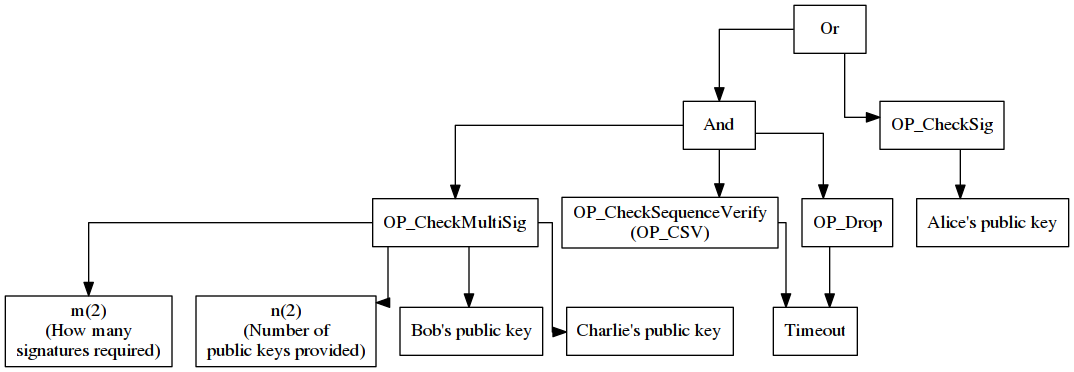
\includegraphics[width=0.8\textwidth]{mast}
    \end{center}
  \item Both \textbf{Schnorr signatures} and a variation of \textbf{MAST} are
    part of the \textbf{Taproot} soft-fork that activated on the mainnet on
    November 14, 2021.
  \end{itemize}
\end{frame}

\begin{frame}
  \frametitle{Second Layer Solutions}
  \begin{itemize}
  \item Perform transactions in a second-layer network and use main Bitcoin
    network (chain) as a settlement layer.
  \item Signed Bitcoin transaction is a payment that can be ``claimed'' by
    publishing it to the Bitcoin network.
  \item Second-layer payments can be implemented with signed Bitcoin
    transactions that are only published when settlement is needed.
  \item Until \textbf{settlement transaction} is published, \textbf{double
      spending} is still possible.
  \end{itemize}
\end{frame}

\begin{frame}
  \frametitle{Payment Channels 1/2}
  \begin{itemize}
  \item \textbf{Payment channel} is a construction that allows \textbf{two}
    parties to transact Bitcoin without submitting any transactions to the
    Bitcoin network.
  \item \textbf{Bidirectional payment channel} is somewhat similar to a payment
    check that splits a joint bank account between two parties.
    \begin{itemize}
    \item joint bank account with ballance N;
    \item both parties A and B ``own'' $N/2$ portions of the ballance;
    \item both parties sign a check that pays $N/2$ money to A and B;
    \item when party A wants to pay $M$ money to party B, they \textbf{sign a
        new check} that pays $N/2 - M$ to party A and $N/2 + M$ to party B and
      \textbf{destroy the old checks}.
    \end{itemize}
  \end{itemize}
\end{frame}

\begin{frame}
  \frametitle{Payment Channels 2/2}
  \begin{itemize}
  \item Several proposals: Spillman, CLTV, Poon-Dryja, Decker-Wattenhofer duplex
    payment channels, Decker-Russell-Osuntokun eltoo Channels.
  \item Poon-Dryja payment channels were presented in the Lightning Network
    paper.
  \item Channel backing funds are locked into a 2-of-2 multisig.
  \item Before the funding transaction is even signed, commitment transactions
    for each party are first written and signed.
  \item As it requires referring to transactions that have not been signed yet,
    it requires using a transaction format that separates signatures from the
    part of the transaction that is hashed to generate the txid, such as
    Segregated Witness.
  \end{itemize}
\end{frame}

\begin{frame}[fragile]
  \frametitle{Lightning Network 1/2}
  \begin{itemize}
  \item A network of bidirectional payment channels that allows to execute
    multi-hop payments, propagating funds through a series of payment channels.
  \item Proposed in 2015, mainnet network started operation in early 2018.
  \end{itemize}
  \begin{center}
    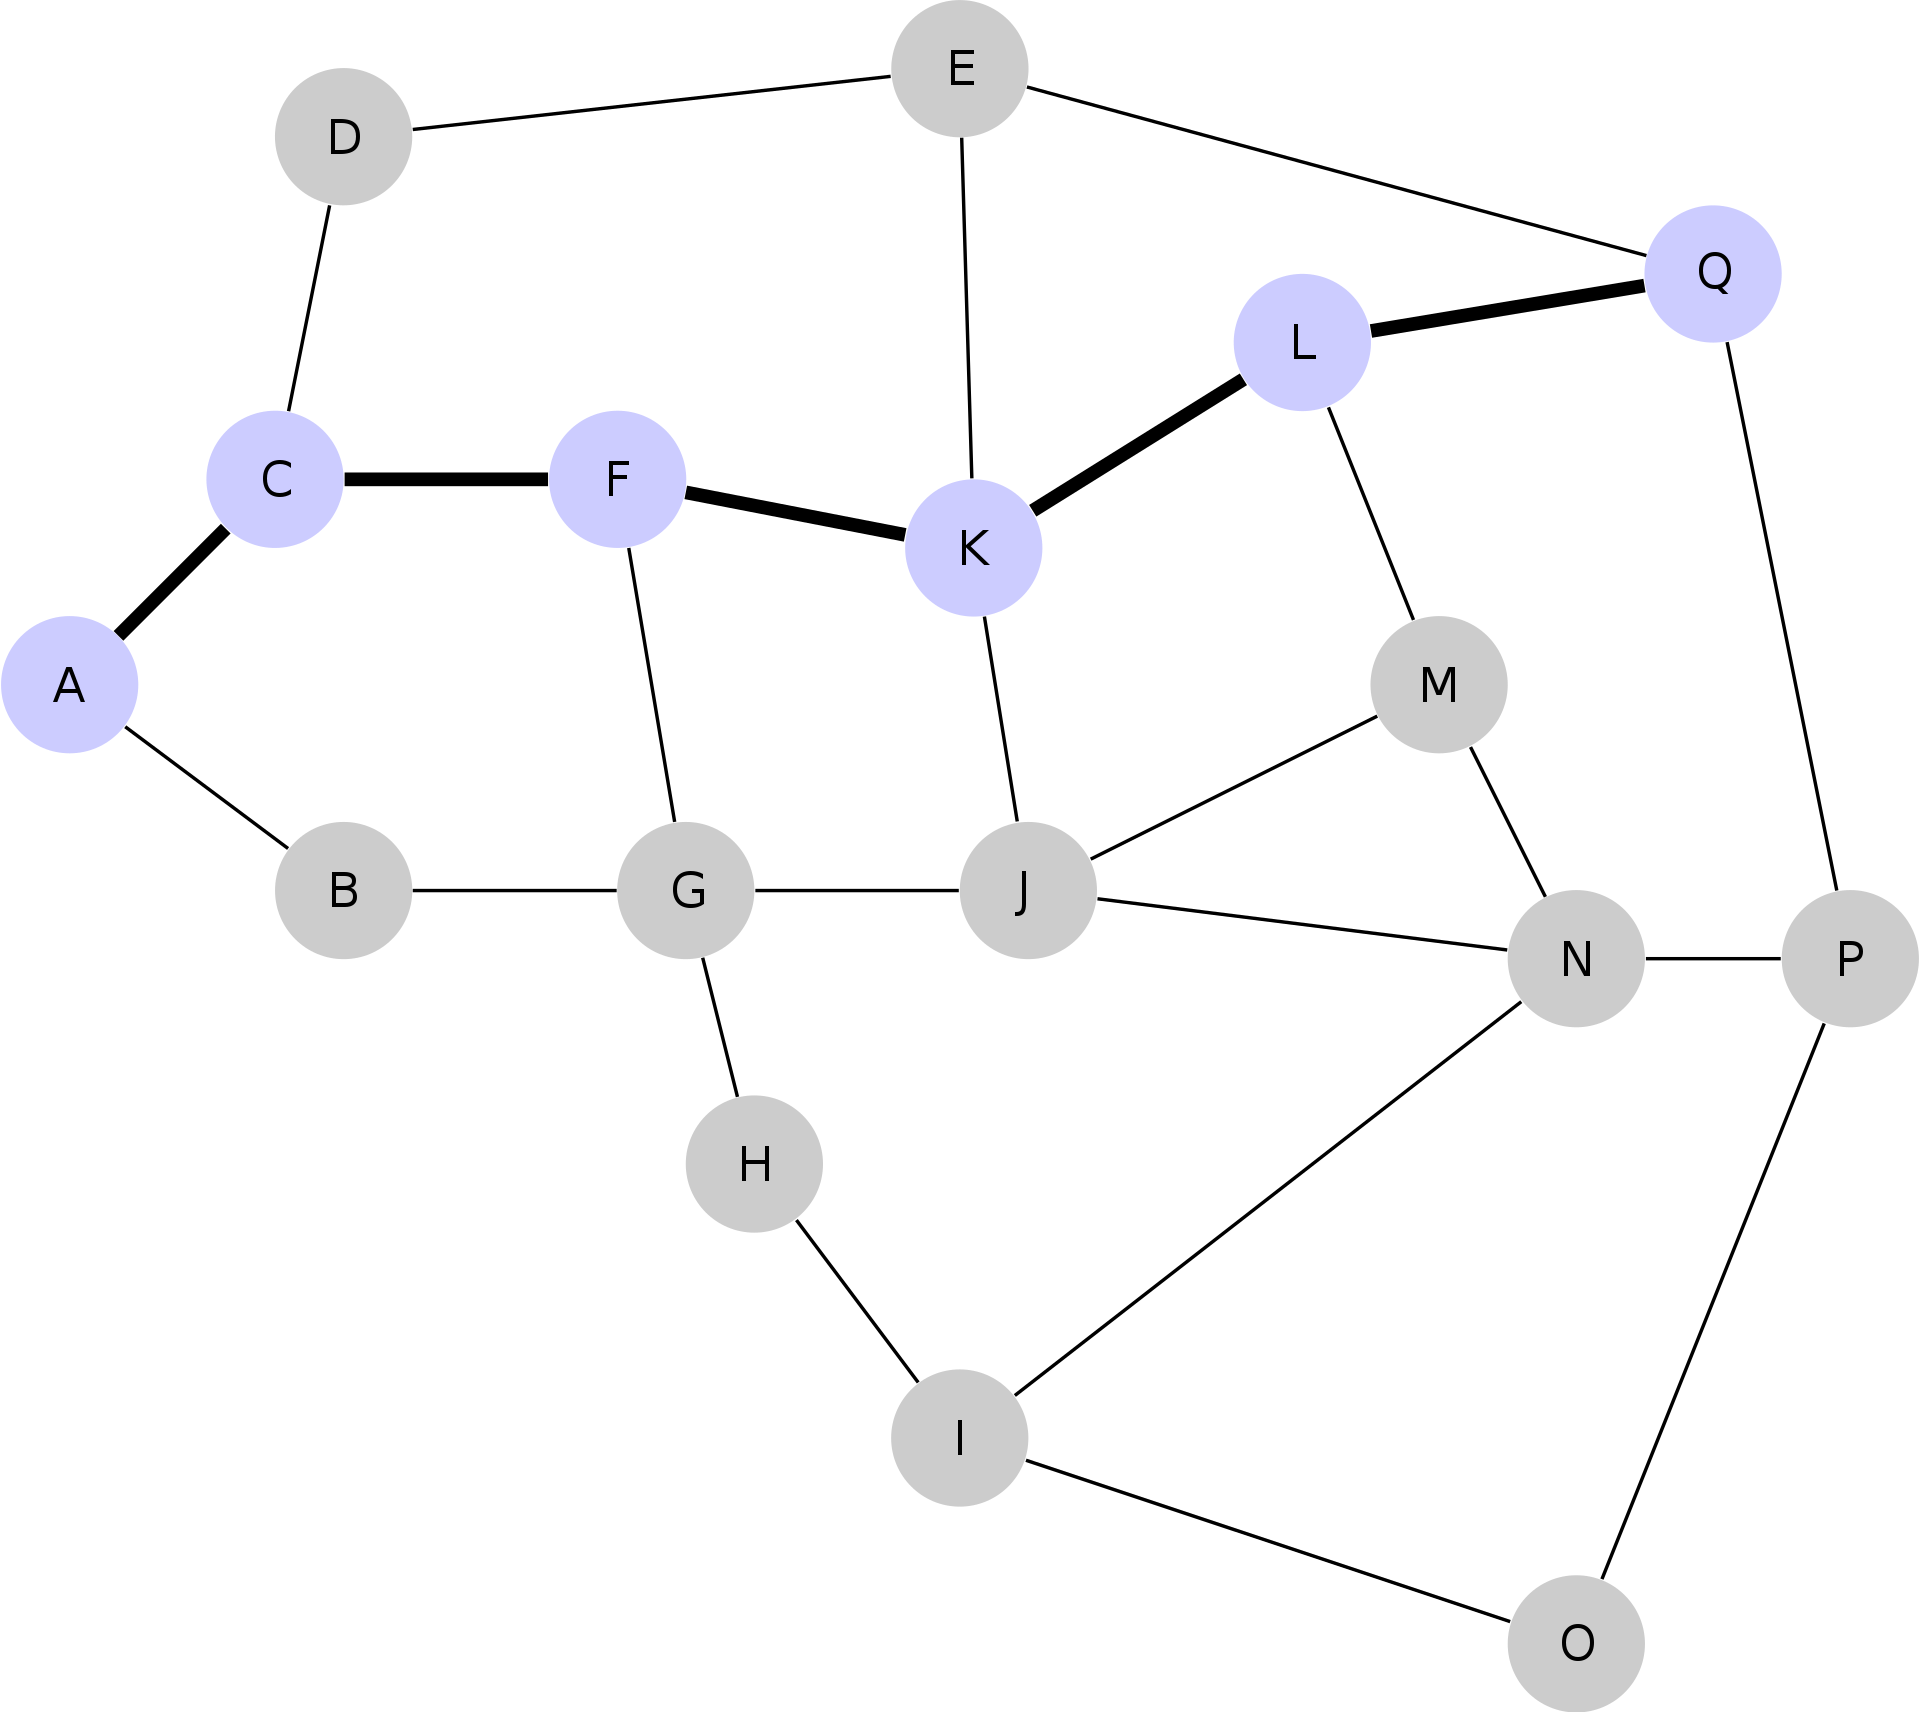
\includegraphics[width=0.5\textwidth]{ln}
  \end{center}
\end{frame}

\begin{frame}[fragile]
  \frametitle{Lightning Network 2/2}
  \begin{itemize}
  \item Entity $A$ wants to pay entity $B$ and there is a path within the network
    between them $A, C_1, C_2, ..., C_n, B$:
    \begin{itemize}
    \item $B$ generates a random value $R$ and computes a hash $H = hash(R)$ and
      provides $H$ to $A$;
    \item $A$ and creates an additional HTLC (Hash Timelock Contract) output and
      updates it's channel with $C_1$:
      \begin{minted}{Lisp}
  IF 
    HASH160 <H> EQUAL
    <B public key> CHECKSIG
  ELSE
    <locktime> CHECKLOCKTIMEVERIFY
    <A public key> CHECKSIG
  ENDIF
      \end{minted}
    \item $C_1$ updates its payment channels with $C_2$ and so on, until $C_n$
      updates channel with $B$.
    \item $B$ provides $R$ to $C_n$ and pulls funds, $C_n$ provides $R$ to
      $C_{n-1}$ and so on until $C_1$ pulls funds from $A$.
    \end{itemize}
  \end{itemize}
\end{frame}

\begin{frame}
  \frametitle{Lightning Network Usage}
  \begin{itemize}
  \item 17,616 nodes (20,478 nodes in 2021),
  \item 84,931 channels (45,774 channels in 2021),
  \item 4,017.60 BTC = \$84,142,806 (1,332.25 BTC = \$52,290,595 in 2021),
  \item Ongoing research, improvements and new feature development,
  \item Games, online shops and other businesses.
  \end{itemize}
\end{frame}

\begin{frame}
  \frametitle{Recommended Resources}
  \begin{itemize}
  \item \textbf{Bitcoin: A Work in Progress}
    \begin{itemize}
    \item book by Sjors Provoost, Bitcoin Core contributor
    \item https://btcwip.com
    \end{itemize}
  \end{itemize}
\end{frame}

\begin{frame}
  \frametitle{The End}
  \begin{center}
    Thank you!
  \end{center}
\end{frame}

\end{document}

%%% Local Variables:
%%% mode: latex
%%% TeX-master: t
%%% End:
